\section{System-FIT}
\label{sec:system_fit}

System-FIT is a framework introduced by \citet{griederDigitalEcosystemHow2019,schwafertsDigitalBusinessDevelopment2020}
and helps companies to evaluate the fit of their business model with an existing or emerging digital ecosystem.
In particular, \cite{schwafertsDigitalBusinessDevelopment2020} argues that most companies are not able
to create their own digital ecosystem and therefore have to join an existing one. The framework
thus helps companies navigate, evaluate and choose the right digital ecosystem to join. 
Further, to be successful in the digital age, companies need to join a digital ecosystem where they can contribute 
to the value co-creation based on their uniqueness \citep{griederDigitalEcosystemHow2019}.
In particular, this thinking allows for companies to \textit{``decouple themselves from the traditional thinking of
company boundaries''} \citep[p.~42]{griederDigitalEcosystemHow2019}.
In the case of career counseling, we have seen in Subsection \ref{subsec:ecosystem} that it
does not meet the definition of a true ecosystem yet. LinkedIn can introduce the CCaaS model to 
create a new digital ecosystem for career counseling as a value co-creation network with LinkedIn
as the most powerful company, i.e., the company of reference at its center. In the following we will thus evaluate
the fit of CCaaS as a transformative business model in the emerging digital ecosystem of AI-based career counseling
using System-FIT. System-FIT uses 5 dimensions to assess the fit of a business model in a digital ecosystem.
The 5 dimensions include \textit{FIT of uniqueness}, \textit{FIT of partnering}, \textit{FIT of management},
\textit{FIT of structure}, and \textit{FIT of customer understanding} and are presented in Figure \ref{fig:system_fit}.

\begin{figure}[h!]
    \centering
    \caption{System-FIT framework, reproduced from \citep[p.~54]{griederDigitalEcosystemHow2019}.}
    \label{fig:system_fit}
    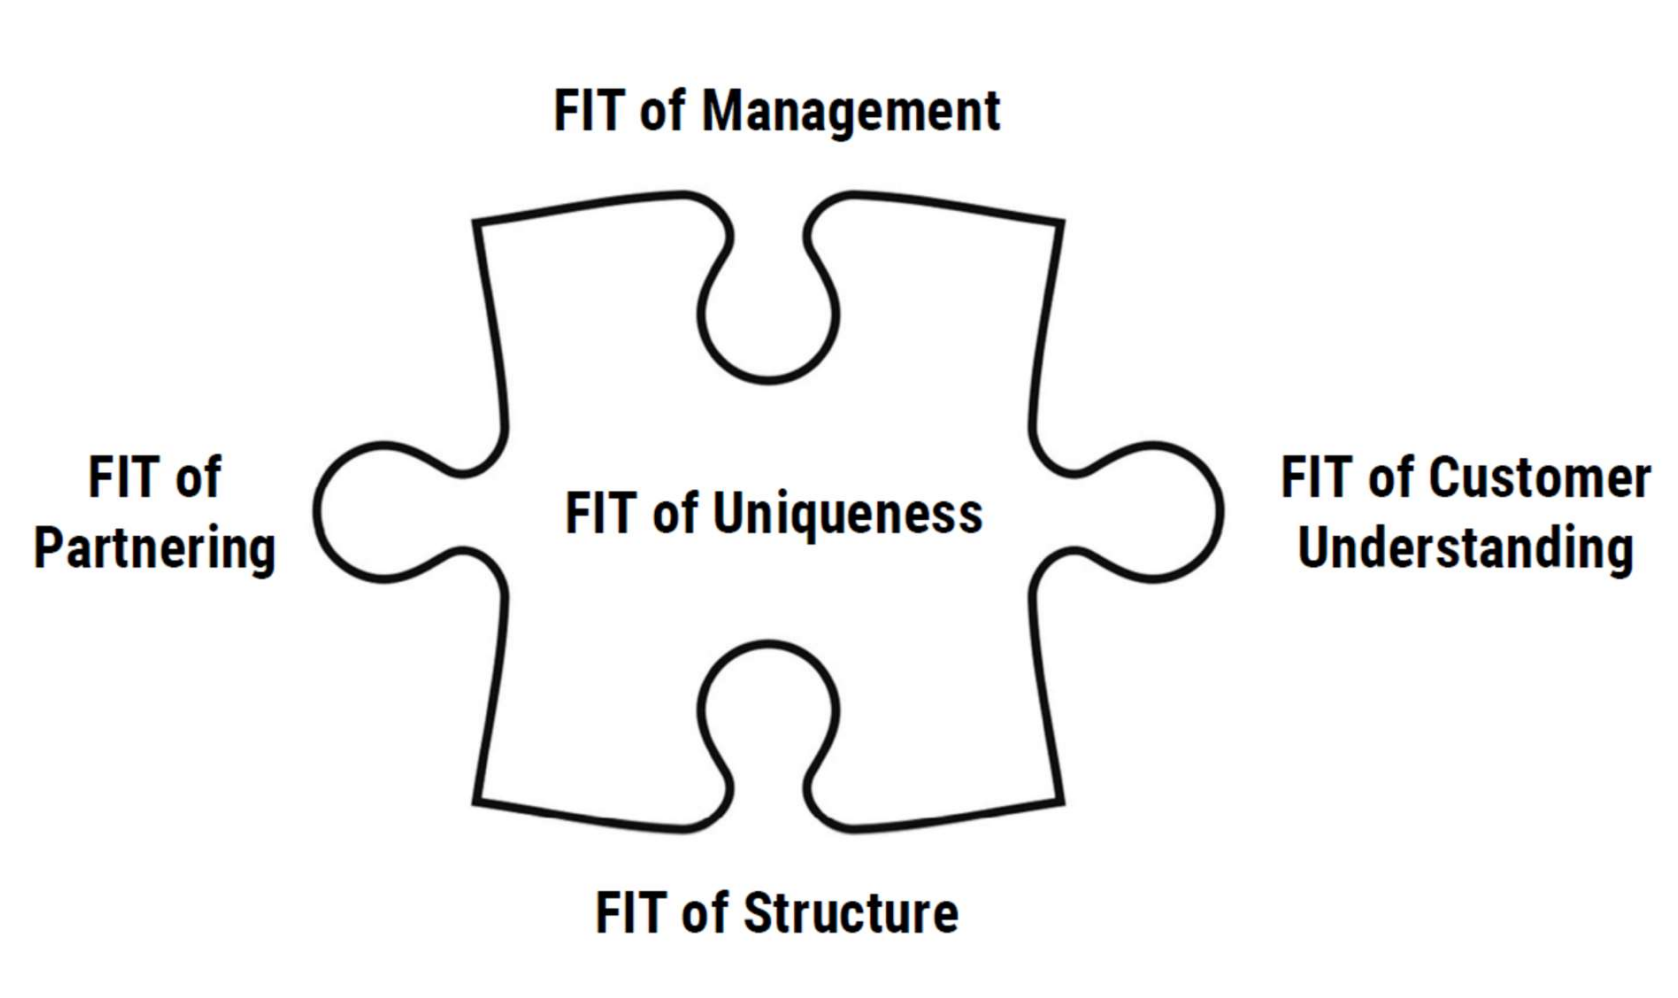
\includegraphics[width=0.7\linewidth]{figures/system-fit.png}
\end{figure}


\subsection{FIT of Uniqueness}

Fit of uniqueness is the understanding of a companies own contribution to the ecosystem, and how it is unique
and cannot be easily replaced---or the value contributed---by competitors \citep[p.~53]{griederDigitalEcosystemHow2019}.
The more unique a company's contribution is, the more it is powerful to influence the ecosystem. The uniqueness of a company's
contribution in a digital ecosystem is determined by its ability to orchestrate the key activities and key resources 
that are required to create a value proposition in the ecosystem \citep[p.~201]{schwafertsLectureStrategicBusiness2023}.

CCaaS is a transformative business model that will create a \textit{new} digital ecosystem for
AI-powered career counseling. The uniqueness of CCaaS is mostly determined by access to data and 
access to machine learning technology. Because LinkedIn is in a ``power play'' position in terms 
of breadth and granularity of employee data, as well as the access to the most advanced AI technology 
through its parent company Microsoft and OpenAI, which Microsoft also invested in.
The key activities of CCaaS are the development and operation of the CCaaS API layer, the development
of the AI-based career counseling algorithms, and the development of the career counseling client
application. The key resources are the data that is required to train the AI-based career counseling
algorithms, the AI technology and the computing resources that are required to run the algorithms and
the CCaaS API layer.

The key activity of "training AI models" is not unique to LinkedIn. However, LinkedIn is a unique position 
through its affiliation with Microsoft and OpenAI to access the most advanced AI technology. The key resource 
of a "large and granular database of employee data" is unique to LinkedIn and cannot be easily replaced by
another company. Based on this analysis, the contribution of LinkedIn to the ecosystem are advanced AI models 
trained on an unparalleled database. For these same reasons, LinkedIn is also the most powerful company in this
emerging digital ecosystem. LinkedIn is needed as the central actor and provider of the CCaaS API platform. It
is unlikely that any other company will be able to create this ecosystem. The need of LinkedIn is thus absolutely
essential.

The uniqueness of the CCaaS model by LinkedIn is limited geographically. While LinkedIn is a global
company, the CCaaS model will only be available in countries where LinkedIn is available and where 
LinkedIn has sufficient user data. Thus, it may happen that another large player appears in other 
markets, such as China and Russia. However, LinkedIn is already the largest professional network in
the world and has a strong brand. It is thus unlikely that another company will be able to compete
with LinkedIn in the foreseeable future in this digital ecosystem. The uniqueness of the contribution 
of the CCaaS model is thus very high, sustainable and LinkedIn as its central actor is confirmed.

\subsection{FIT of Partnering}

Fit of partnering is the companies understanding of the value co-creation chain in the digital
ecosystem, an understanding of its participants, and its alignment with the ethics and values that prevail
in the same \citep[p.~53]{griederDigitalEcosystemHow2019}.

According to \citet{kaserAIpoweredCareerCounseling2023}, ethical consideration in AI-powered career counseling 
include: bias ingrained in AI models, authoritarianism and lack of explainability of AI models, and 
Kafkaesque interactions between the clients and machines. The CCaaS model is designed to address these ethical
concerns. Because the concerns can not be addressed directly in the AI models (but root in these same models),
LinkedIn is reliant on the career counselor to interpret the results of its AI models. Thus, the value
co-creation for the end customer is a symbiosis of AI supplied by LinkedIn's CCaaS and human interpretation by
the career counselor. The career counselor is thus a key partner in the CCaaS model.
Through leveraging the co-creation in the ecosystem, CCaaS can circumvent bias, authoritarianism, 
lack of explainability and Kafkaesque interactions as the career counselor can contribute with his 
human intelligence to overcome these issues.

The new and emerging digital ecosystem of AI-based career counseling thus fully relies on value co-creation.
The ecosystem actors are thus partners and each contribute
to the value that is created for the counseling clients. Using feedback data from the counselors and
clients, the value proposition can be enhanced, and the ecosystem actors can further improve their
offerings: the sum of co-created value thereby surpasses the value creation that each actor could
achieve on its own. The ecosystem actors are thus interdependent and rely on each other. Using a
human in the loop approach as a fundamental ethical value, LinkedIn and career counselors can align
on the ultimate goal of providing the best possible career outcomes for the counseling clients,
without LinkedIn threatening the jobs of the career counselors through automation. The emerging
digital ecosystem will thus be very stable as LinkedIn will be the uncontested central actor, all 
while being dependent on counselors, e.g., to provide local physical presence. The ecosystem actors
will thus be able to rely on the ecosystem and invest in their offerings. The CCaaS model will also
allow for a high degree of customization and thus enable the ecosystem actors to differentiate their
offerings. The pricing of the API is fair and transparent, although limited competition between
different career counselors could arise. However, this competition is likely to improve the quality
of the offerings and/or drive down the costs for the counseling clients. 

\subsection{FIT of Management}

As part of the fit of management, the company needs to assess if its value creation will be accepted by
the most powerful company in the ecosystem, and if it aligns with the ecosystem governance
\citep[p.~53]{griederDigitalEcosystemHow2019}.

In the emerging digital ecosystem of AI-based career counseling, LinkedIn itself is the most powerful company.
LinkedIn is also the orchestrator of the ecosystem via its CCaaS model. Thus, LinkedIn has the power 
to establish the rules of the ecosystem and to steer the direction of development of the ecosystem. In 
particular, LinkedIn can exclude other actors from the CCaaS API layer thereby limiting their ability
to provide good counseling and recommendations to their clients. Thus, LinkedIn governs the rules of 
alignment in the ecosystem. As such, LinkedIn can drive the development of the ecosystem and define 
the pace of development and innovation. However, as career counseling revolves around personal data,
privacy and data protection are important aspects that are dictated by the regulators. Thus, LinkedIn
is not completely free to define the rules of the ecosystem. For instance, LinkedIn may be forced to
offer a "local" version of CCaaS on the European market due to raising incompatibility between business 
practices in the United States with Europe's GDPR legislation.

The management of LinkedIn should therefore consider the other actors in the digital ecosystem, the clients 
and the regulators and each of these actors' needs.
In particular, the needs and pains of career counselors and clients need to be integrated into the decision-making
processes. As argued previously, the CCaaS model relies on value co-creation and thus requires strong 
partners that are enabled to innovate via the CCaaS API layer, but also help to overcome limitations and ethical 
concerns introduced by AI. This form of open innovation will also 
benefit LinkedIn through increased usage of the CCaaS API that will lead to higher revenues and more
feedback data. LinkedIn thus has to act as the orchestrator of the emerging digital ecosystem and
ensure proper governance (such as same access and pricing conditions for all players). This will build
multilateral trust, lead to alignment of the ecosystem actors and ultimately facilitate and accelerate
the joint value-creation. With a steadily increasing workforce with tertiary education in the Western
world, the demand for counseling services will continue to grow. The digital ecosystem will thus 
provide plenty of opportunities for many actors to co-create value and grow together.


\subsection{FIT of Structure}

Fit of structure refers to the companies understanding and (technical) ability to implement solutions
that seamlessly integrate with the digital ecosystem \citep[p.~53]{griederDigitalEcosystemHow2019}. 

The (infra-)structure of the digital ecosystem does not exist yet. However, LinkedIn has the
data and access to the computation and AI technology resources via its parent company Microsoft. As
introduced in subsection \ref{subsec:system_architecture}, the system architecture of CCaaS is based 
on a microservice architecture. This allows for a modular and flexible system structure that can be
easily adapted to the needs of the ecosystem actors as well as to evolving needs: new microservices 
may easily be added while microservices that are no longer needed could be retired. Of course---referring 
back to Fit of Management---LinkedIn has to be cautious in taking decisions to retire microservices 
and consider the needs of the ecosystem actors.

As LinkedIn will be the provider of the CCaaS API layer, it can actually also consider the fit of
structure of the ecosystem actors. By doing this, LinkedIn gains an understanding how it can design 
its CCaaS API layer in a way that can be easily adopted by and integrated into the ecosystem actors'
systems. Therefore, the CCaaS API layer should be well documented, easy to use, be kept as stable
as possible, and backwards-compatible to ensure that the ecosystem actors can rely on it. Any changes
to the API  or removing of services have to be planned well in advance and communicated to the ecosystem
actors to give them enough time to adapt. Ideally the CCaaS API layer will be extended over time to provide
more functionality and thus enable the ecosystem actors to innovate and create more value. Through
the API-based architecture, other actors in the ecosystem are empowered to customize their own offerings.



\subsection{FIT of Customer Understanding}

Finally, fit of customer understanding refers to the company's ability to understand the expectations 
of customers as well as the ethics and values that prevail in the ecosystem \citep[p.~53]{griederDigitalEcosystemHow2019}.

In the case of LinkedIn's CCaaS, the final customers and beneficiaries of the value creation are the
counseling clients. As we mentioned before, the introduction of AI in the career counseling process
will lead to ethical concerns and issues. In particular, the lack of explainability of AI-based
recommendations and the potential for bias in the data and algorithms are important issues that 
ultimately affect the counseling clients. The career counselors can help to overcome these issues by providing
a human in the loop approach, i.e., by acting as an interface between the AI provided in CCaaS and the 
humans. The career counselors can explain the recommendations to the clients, and make sure that the 
recommendations are not suffering bias. 

LinkedIn's CCaaS offering is thus fully complementary to existing career counselors' services. The CCaaS
addresses pains and potential gains of counseling clients that the counselors alone cannot tackle 
(such as providing affordable career advice, more personalized coaching, and reducing risks 
in career transitions through better AI-based insights on LinkedIn's data). On the other hand, career 
counselors provide the human in the loop that addresses the ethical issues rooted in AI models. The symbiosis
of CCaaS and counselors thus act in the best interest and according to the expectations of counseling clients,
which will lead to a high degree of customer satisfaction.
\newline

\noindent The final Section \ref{sec:conclusion} will summarize and discuss the findings from 
this paper.
